% Created 2024-06-19 mié 01:17
% Intended LaTeX compiler: pdflatex
\documentclass[presentation]{beamer}
\usepackage[utf8]{inputenc}
\usepackage[T1]{fontenc}
\usepackage{graphicx}
\usepackage{grffile}
\usepackage{longtable}
\usepackage{wrapfig}
\usepackage{rotating}
\usepackage[normalem]{ulem}
\usepackage{amsmath}
\usepackage{textcomp}
\usepackage{amssymb}
\usepackage{capt-of}
\usepackage{hyperref}
\usetheme{Madrid}
\usecolortheme{}
\usefonttheme{}
\useinnertheme{}
\useoutertheme{}
\author{Luis Enrique Perez Señalin}
\date{\textit{<2024-06-05 mié>}}
\title{Circuitos combinatorios}

\hypersetup{
 pdfauthor={Luis Enrique Perez Señalin},
 pdftitle={Circuitos combinatorios},
 pdfkeywords={},
 pdfsubject={},
 pdfcreator={Emacs 27.1 (Org mode 9.3)}, 
 pdflang={Spanish}}
\begin{document}

\maketitle
\begin{frame}{Outline}
\tableofcontents
\end{frame}


\section{Ejercicios}
\label{sec:org5f0dcd4}
\begin{frame}[label={sec:org4e7f694}]{Ejercicio1}
\begin{center}
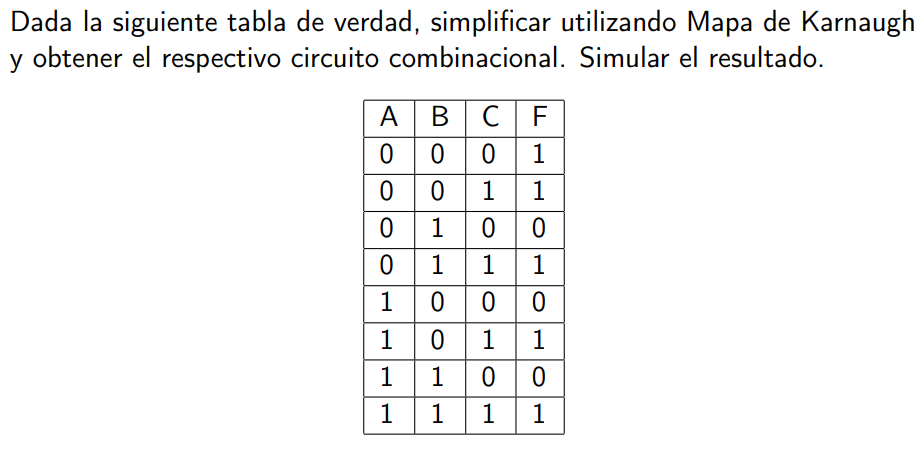
\includegraphics[width=.9\linewidth]{./ejercicio1.png}
\end{center}
\end{frame}

\begin{frame}[label={sec:org93bc206}]{Ejercicio2}
\begin{center}
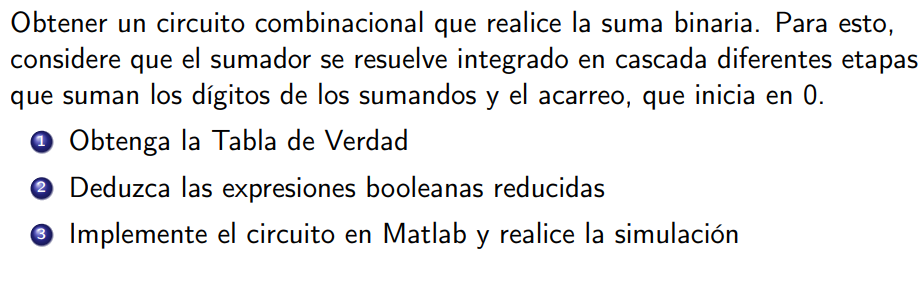
\includegraphics[width=.9\linewidth]{./ejercicio2.png}
\end{center}
\end{frame}

\section{Resolución}
\label{sec:orgc9c04f5}

\begin{frame}[label={sec:org369314a}]{Ejercicio 1 - 1}
\begin{center}
\begin{tabular}{|l|l|l|l|}
\hline
A & B & C & F \\
\hline
0 & 0 & 0 & 1 \\
\hline
0 & 0 & 1 & 1 \\
\hline
0 & 1 & 0 & 0 \\
\hline
0 & 1 & 1 & 1 \\
\hline
1 & 0 & 0 & 0 \\
\hline
1 & 0 & 1 & 1 \\
\hline
1 & 1 & 0 & 0 \\
\hline
1 & 1 & 1 & 1 \\
\hline
\end{tabular}
\end{center}
\end{frame}

\begin{frame}[label={sec:orgcdeb460}]{Ejercicio 1 - 2}
Mapa de Karnaugh
\begin{center}
\begin{tabular}{|l|l|l|l|l|}
\hline
AB/ & 00 & 01 & 11 & 10 \\
C & & & & \\
\hline
0 & 1 & 0 & 0 & 0 \\
\hline
1 & 1 & 1 & 1 & 1 \\
\hline
\end{tabular}
\end{center}

$$F = \overline{ABC} + C$$
\end{frame}

\begin{frame}[label={sec:orgaed0439}]{Ejercicio 1 simulacion}
\begin{center}
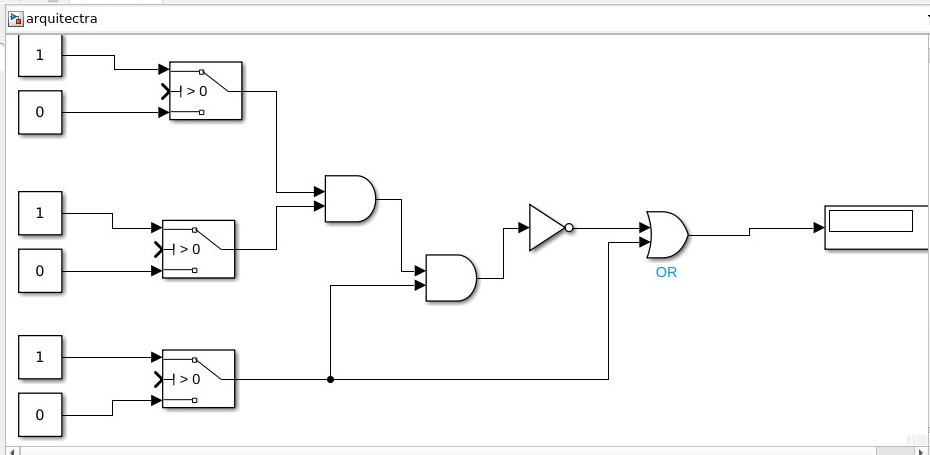
\includegraphics[width=.9\linewidth]{./ejercicio1_simulacion.png}
\end{center}
\end{frame}

\begin{frame}[label={sec:org3d2a8b7}]{Ejercicio 2}
Obtener la tabla de verdad:
\begin{center}
\begin{tabular}{|l|l|l|l|l|}
\hline
A & B & C & S & C \\
\hline
0 & 0 & 0 & 1 & 0 \\
\hline
0 & 0 & 1 & 1 & 0 \\
\hline
0 & 1 & 0 & 1 & 0 \\
\hline
0 & 1 & 1 & 0 & 1 \\
\hline
1 & 0 & 0 & 1 & 0 \\
\hline
1 & 0 & 1 & 0 & 1 \\
\hline
1 & 1 & 0 & 0 & 1 \\
\hline
1 & 1 & 1 & 1 & 1 \\
\hline
\end{tabular}
\end{center}
\end{frame}

\begin{frame}[label={sec:org0fdba76}]{Ejercicio 2 - expresion booleana}
Deducir las expresiones booleanas reducidas

Para S, usamos la operación XOR:
\(S = A(+)B(+)C\)

Para C(acarreo), utilizamos:
\(C = (A*B) + ( C*(A(+)B) )\)
\end{frame}

\begin{frame}[label={sec:orga1dc57d}]{Ejercicio 2 - simulacion}
\begin{center}
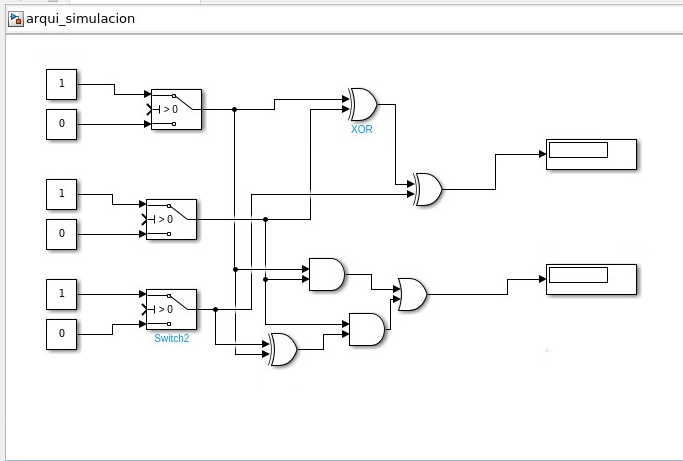
\includegraphics[width=.9\linewidth]{./ejercicio2_simulacion.png}
\end{center}
\end{frame}
\end{document}
